\skiptooddpage
\section{Totálisan unimoduláris mátrixok és alkalmazásai}

Egy totálisan unimoduláris mátrixon minden négyzetes részmátrixának determinánsa
$0, 1$ vagy $-1$. Ehhez szükséges (de nem elégséges) feltétel, hogy a mátrix
elemei is csak $0, 1$ vagy $-1$ lehetnek.

\[
\begin{rcases}
A \text{ totálisan unimoduláris -- TU} \\
b \text{ egész vektor} \\
c \text{ tetszőleges} \in \mathbb{R}^n \\
\text{max} \left\{ cx:Ax \leq b \right\} \text{ LP feladat}\\
\text{ami megoldható és felülről korlátos}
\end{rcases} \Rightarrow \parbox[t]{8cm}{ Az IP feladat is megoldható és az LP
feladat maximuma megegyezik az IP feladat maximumával.} \]

\emph{Lemma:} a totálisan unimoduláris tulajdonság megmarad, ha:

\begin{description}
\item[sor vagy oszlopot $\cdot (-1)$] $\Rightarrow$ ekkor a determináns
előjele változik meg.
\item[egységvektor sor vagy oszlopként való hozzáadása] $\Rightarrow$ ha a
mátrixhoz egységvektort veszünk hozzá például oszlopként, és egy kiválasztott
négyzetes részmátrixában ez az oszlop szerepel, akkor az új oszlop szerinti
kifejtésből azonnal látszik, hogy a determináns megegyezik az eredeti mátrix
egy négyzetes részmátrixának determinánsával vagy annak ellentettjével, így
értéke $0, 1$ vagy $-1$.
\item[sor vagy oszlop ismétlés] $\Rightarrow$ ha a kiválasztott részmátrixba
az eredeti is szerepel a determináns nulla lesz, ha csak az egyik marad, akkor
előáll az eredeti mátrixból képzett részmátrix, amely determinánsának értéke
megmarad $0, 1$ vagy $-1$.
\item[transzponáljuk] $\Rightarrow$ megmarad a determináns definíciójának
következményeként.
\end{description}

\emph{Tétel. Bármely irányított gráf illeszkedés mátrixa~\footnote{$
B(G_{(V,E)})=
b_{i_{\in V}j_{\in E}}=
\begin{cases}
0  & \text{ha a } j \text{--edik él nem illeszkedik az } i \text{--edik ponthoz,} \\
+1  & \text{ha a } j \text{--edik élnek az } i \text{--edik pont kezdőpontja,} \\
-1  & \text{ha a } j \text{--edik élnek az } i \text{--edik pont a végpontja,} \\
+1  & \text{ha a } j \text{--edik él az } i \text{--edik ponthoz illeszkedő hurokél.} \\
\end{cases}$} totálisan unimoduláris.}.
\vspace{0.4cm}

Irányított illeszkedési mátrixnál az oszlopban $1$ van, amely pontból indul az
él, $-1$ ahova mutat; hurok--él esetében egyetlen $1$--es található. A
bizonyítás teljes indukcióval. Legyen $M \in \mathbb{M}_{k\times k}$ méretű
részmátrix. Ha $k=1$ az állítás nyilvánvaló. Ha $k \geq 2$ és létezik egy darab
oszlop, amelybe legfeljebb egy nem nulla elem van, akkor kifejtés a szerint és
az indukció adja a többit (a kifejtés alapján $-1\cdot detM_{n-1\times n-1}$
lesz a determináns, ami $1,0$ vagy $-1$).

Másképp minden oszlopában egy darab $+1$ és egy darab $-1$ van, és a többi
nulla. Így $M$ sorainak összege null vektor, előállítható mint nem triviális
lineáris kombináció, azaz a sorok összefűggöek, és ezért $\Rightarrow$ det$M=0$.

\subsection{Maximális összsúlyú párosítás IP feladatként}

\emph{Tétel. Páros gráf~\footnote{Páros gráfnak nevezünk egy $G$ gráfot, ha
csúcsainak halmazát fel tudjuk úgy osztani egy $A$ és $B$ halmazra, hogy az
összes $G$-beli élre teljesül, hogy az egyik végpontja $A$-ban van, a másik
pedig $B$-ben.} illeszkedési mátrixa totálisan unimoduláris.}
\vspace{0.4cm}

Mutasson minden él $A$--ból $B$--be. Irányított gráf illeszkedési mátrixa TU. Az
eredeti illeszkedési mátrixának megkapásához $B$ csúcsainak megfelelő sorokat
$-1$--el szorozzuk.

Legyen $x$ indikátor, hogy az él benne van-e párosításban, $w$ egy tetszőleges
él súlyfüggvény és $B$ az illeszkedési mátrix (amely páros gráf lévén totálisan
unimoduláris). A \emph{feladat}, megfogalmazható, mint max$\left\{ wx:Bx \leq (1,
\cdots, 1)^T, x \geq 0 \right\}$. Az $x \geq 0 $ feltételt bevisszük $B$
mátrixba kiegészítve azt egy $m \times m$--es egységmátrix ellentettjével, de ez
nem változtat TU tulajdonságon.

Az egyenlőtlenség így azt fejezi ki, hogy egy csúcsból legfeljebb egy kiinduló
élet választunk ki, ami adja a párosítás feladatát.

\[
\begin{rcases}
B'=\begin{bmatrix} ~~B \\ -I \end{bmatrix} \text{ TU} \\
b \text{ egész}
\end{rcases} \Rightarrow x \text{ egész vektor ($0$ vagy $1$) értékű -- IP feladat}
\]

A max$\left\{ wx : Bx \leq (1,\cdots,1)^T, x \geq 0 \right\}$ duálisa
min$\{ y(1,\cdots,1)^T : yB \geq w,$ $y~\geq~0\}$. Az $y$ megoldás
minden $v$ csúcshoz $c(v)$ címkét rendel, ahogy Egerváry Jenő párosítás
algoritmusa is:

\[ yB \geq w \Rightarrow c(a) + c(b) \geq w(e), \forall e=\{a,b\}\in E.\]

\subsection{Intervallumgráf}

A számegyenes véges sok intervalluma alkossa egy gráf csúcshalmazát, és két
csúcs akkor legyen szomszédos, ha a megfelelő intervallumok metszők; az így
meghatározott gráf az intervallumgráf. Feltehető, hogy a gráfot meghatározó
intervallumok $n$--re az $[1,n]$ egész végpontú, zárt részintervallumai.
Legyen az $I=\left\{I_1, I_2, \cdots, I_m\right\}$ intervallumrendszer.

Rendeljük ehhez $n \times m$--es $A(I)$ mátrixot: sorai feleljenek meg az
$1,2,\cdots,n$ egészeknek, oszlopai pedig az I intervallumainak. Az $i$--ik sor
és a $j$--ik oszlop kereszteződésben akkor álljon $1$--es, ha $i \in I_j$, és
minden más helyen álljon $0$.

\begin{figure}[htbp]
\centering
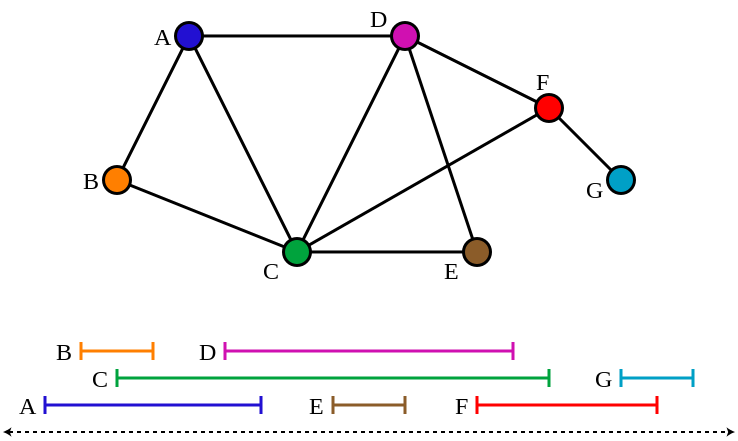
\includegraphics[width=0.8\textwidth]{./kepek/intervalum_graf.png}
\caption{Példa intervallum gráfra} \label{fig:int_graf}
\end{figure}

\emph{Tétel. Az így definiált A(I) mátrix totálisan unimoduláris.}
\vspace{0.4cm}

A bizonyításhoz kiválasztunk egy tetszőleges $k \times k$ részmátrixot, majd
teljes indukciót használunk az egyesek darabszáma szerint. Ha nulla darab
egyesből áll a mátrix az nyilván TU. Ha van benne két oszlop, amelyben az első
egyes azonos helyen áll, akkor a nagyobb egyes darabszámúból kivonjuk a kisebb
darabszámot. Ez az egyesek darabszámát csökkenti, de a determinánsát nem
változtatja.

Ha nincs ilyen oszlop, de van csupa nulla oszlop, akkor a determináns nulla. Ha
egyik sem teljesül, akkor pedig be tudjuk rendezni az oszlopokat úgy, hogy az
alsóháromszög mátrixot kapunk oszlop cserével. Ez a művelet a determinánst csak
előjelben változtatja meg, így a determináns $1$ vagy $-1$ marad.
\vspace{0.4cm}

\emph{Tétel. Az intervallumgráfok tetszőleges k színre megszínezhetőek
egyenletesen.}
\vspace{0.4cm}

Az ``egyenletesen'' alatt azt értjük, hogy ha $i$--t tartalmazó intervallumok
száma $d_i$, akkor ezek közül minden felhasznált szín esetén az ilyen színű
intervallumok száma $\lceil \frac{d_i}{k} \rceil$~\footnote{felső egész rész}
vagy $\lfloor \frac{d_i}{k} \rfloor$~\footnote{alsó egész rész}.

Elég bebizonyítani, hogy az intervallumok közül kiválasztható néhány úgy, hogy
bármely $1 \leq i \leq n$ esetén az $i$--t tartalmazó intervallumok között
$\lceil \frac{d_i}{k} \rceil$ vagy $\lfloor \frac{d_i}{k} \rfloor$ darab
kiválasztott intervallum legyen. Ekkor a kiválasztott intervallumokat
megszínezzük egy színnel, majd elhagyjuk őket. A megmaradt intervallumra meg
ugyanaz $k-1$--el és így tovább.

Legyen:
\[\begin{rcases}
A=A(I) \mbox{ intervallumokhoz rendelt mátrix}\\
d = n \text{ dimenziós vektor } i \text{--ik komponense } d_i \\
\lceil \frac{d}{k} \rceil \text{ vektor } i \text{--ik komponense} \lceil \frac{d_i}{k} \rceil \\
\lfloor \frac{d}{k} \rfloor \text{ vektor } i \text{--ik komponense} \lfloor
\frac{d_i}{k} \rfloor \\
\lfloor \frac{d}{k} \rfloor \leq Ax \leq \lceil \frac{d}{k} \rceil, 0 \leq x
\leq (1,\cdots, 1)^T \end{rcases} \parbox[L]{6cm}{Erre nyilvánvalóan megoldás az
$x~=~\left( \frac{1}{k}, \cdots, \frac{1}{k} \right)^T$ de tudjuk, hogy $A$ TU
$\Rightarrow \exists$ egészértékű megoldása is .}
\]

Legyen $x$ ez az egész értékű vektor, $0$ vagy $1$ elemeket tartalmaz, és az
$1$--es komponenseknek megfelelő oszlopok összege $\lceil \frac{d}{k} \rceil$ és
$ \lfloor \frac{d}{k} \rfloor$ között van. Így ezeknek az oszlopoknak megfelelő
intervallumukat kiválasztva valóbban $\lceil \frac{d_i}{k} \rceil$ vagy $
\lfloor \frac{d_i}{k} \rfloor$ illeszkedik $i$--re.

A tétel következménye, hogy az intervallumgráfok \emph{perfektek}~\footnote{ Egy
gráfot akkor nevezünk \emph{perfektnek} ha rá és minden F feszített részgráfjára
teljesül, hogy $\chi(F) = \omega(F)$, azaz a kromatikus szám~\footnotemark{}
megegyezik a maximásis klikkmérettel.}\footnotetext{$k$ színnel kiszinezhető de
$k-1$--el már nem, ahol a kiszinhezhetőség azt jelenti, hogy minden csúcsot ki
lehet színezni $k$ színnel úgy, hogy szomszédos csúcsók között nincs egyforma
szinű} (feltéve, hogy az intervallumgráf minden részgráfja is intervallumgráf).
Ez igaz, mivel legyen $k=\omega(G)$. Ekkor alkalmazva a fenti tételt azt kapjuk,
hogy a csúcsok jól színezhetőek $k$ színnel, vagyis $\omega(G)=\chi(G)$.